\chapter{Design}
	
	After the security audit, it was apparent that the majority of the codebase needed to be refactored in order to make it object-oriented.
	The decision to rewrite the program was not a light one, by rewriting the program, the scope of extensions to \ac{AWESOME} became much more limited via time constraints.
	
	With the rewrite came the opportunity to utilise both a framework and a design pattern.
	Frameworks were ruled out under the stance that it had to be deployed on a server without shell access.
	However later research discovered that this is achievable in Laravel\footnote{Laravel Homepage: \url{http://laravel.com}}, which would have been the framework of choice for several reasons.
	
	Laravel would have provided a complete, and mature \ac{MVC} framework, as well as an \ac{i18n} framework and a solid basis for \ac{AWESOME}.
	Ultimately, poor research into Laravel on a shell-less server resulted in an attempt to produce a bespoke \ac{MVC} framework, which, unsurprisingly is harder than it first seems.
	
	\section{Programming Language}
	
	The programming language choice was fairly fixed, as it had to be easily runnable on an \ac{AU} server.
	This limited the choice to PHP, but which minor version of it was only found out later in the project which is discussed further in \autoref{sec:implementation}.
	
	If this requirement wasn't an issue, Ruby on Rails would have been the ideal candidate for this project, as it already provides an \ac{MVC} framework and gems for \ac{i18n}.
	
	\section{\acl{MVC} Framework}
	
	Since using a framework was ruled out, a custom-made \ac{MVC} framework was written to support this project.
	The design of which is laid out in this section and is very heavily taken from the `Write your own PHP MVC Framework' series of tutorials\cite{php-mvc-tutorial}.
	
	
	\section{Internationalisation Framework}
	
	The \ac{i18n} framework is a standalone \ac{OOP} module which utilises JSON formatted files with strings for translation.
	
	\section{Database Schema}
	
	\section{User Interface}
	
	The user interface was fairly good on the questionnaire-side in the prototype, so a lot of elements were re-used in that, with a few minor changes.
	
	\autoref{fig:questionnaire-comparison} shows a comparison between the prototype version and the submitted version of \ac{AWESOME}.
	
	\begin{figure}[h]
		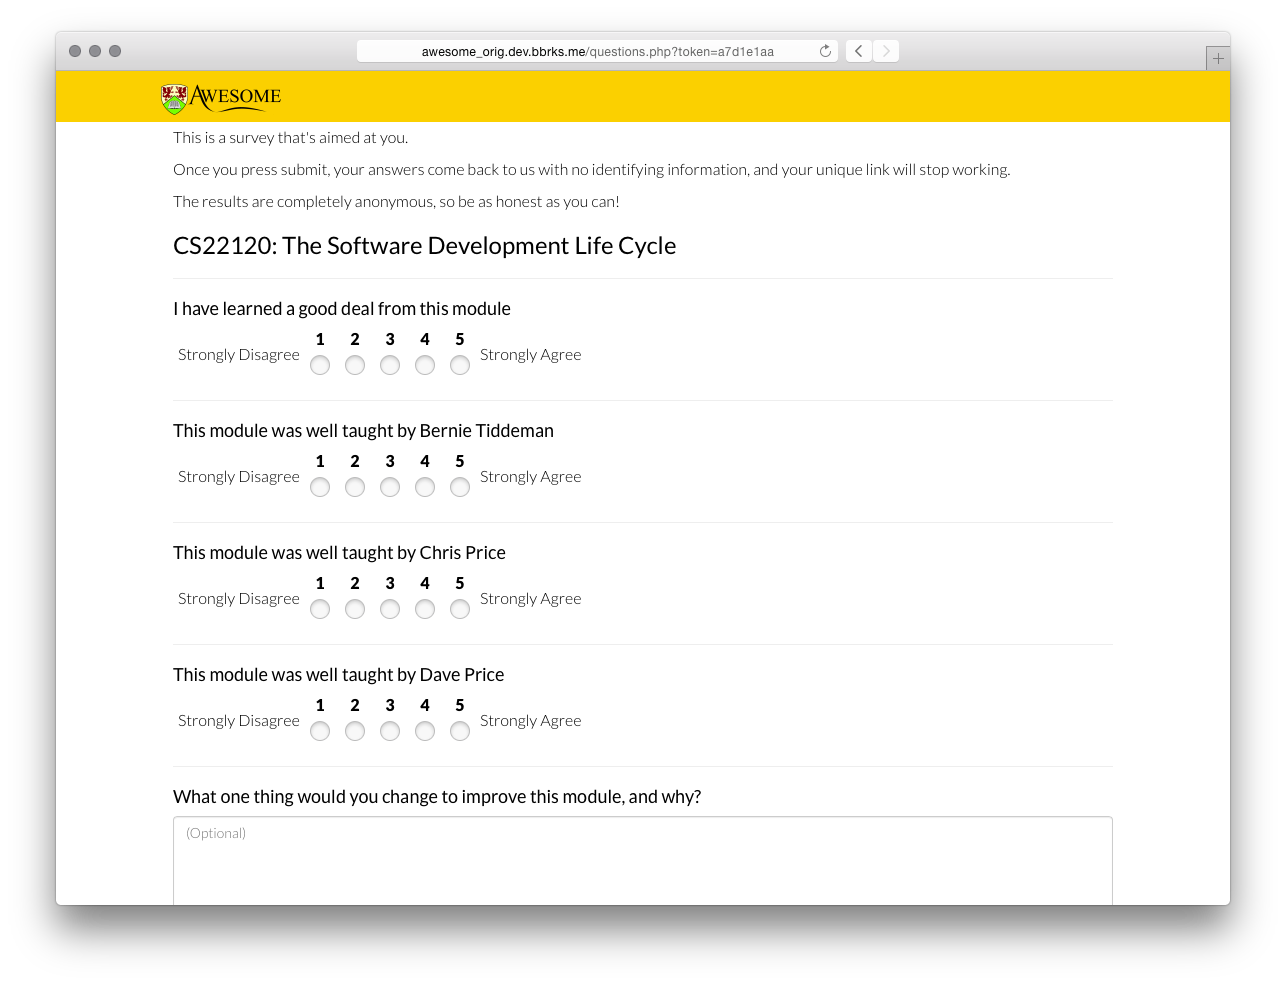
\includegraphics[width=\textwidth]{screens/prototype-questionnaire}
		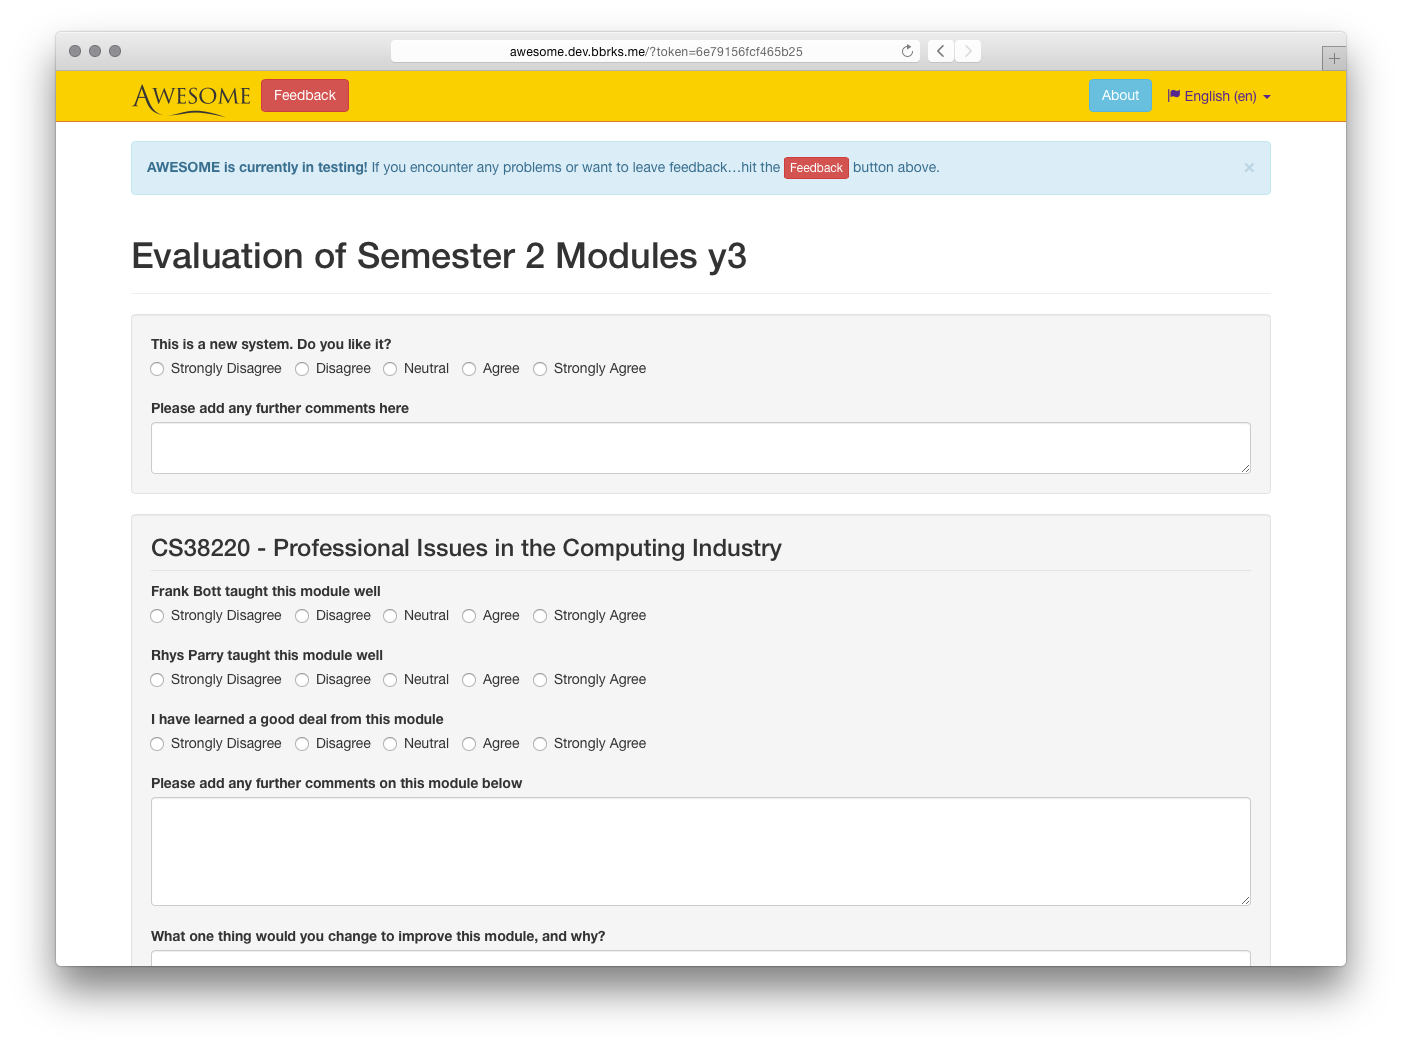
\includegraphics[width=\textwidth]{screens/final-questionnaire}
		\caption{A comparison of questionnaire pages between the prototype version and the submitted version of \acs{AWESOME}}
		\label{fig:questionnaire-comparison}
	\end{figure}
	
	The admin dashboard of the prototype wasn't very user friendly.
	Creating surveys, adding questions, modules, students, and staff was fairly convoluted.
	Results weren't clear to look at, and took up a lot of space per-question by pie charts, which were unnecessary given the data provided.
	
	\begin{figure}[h]
		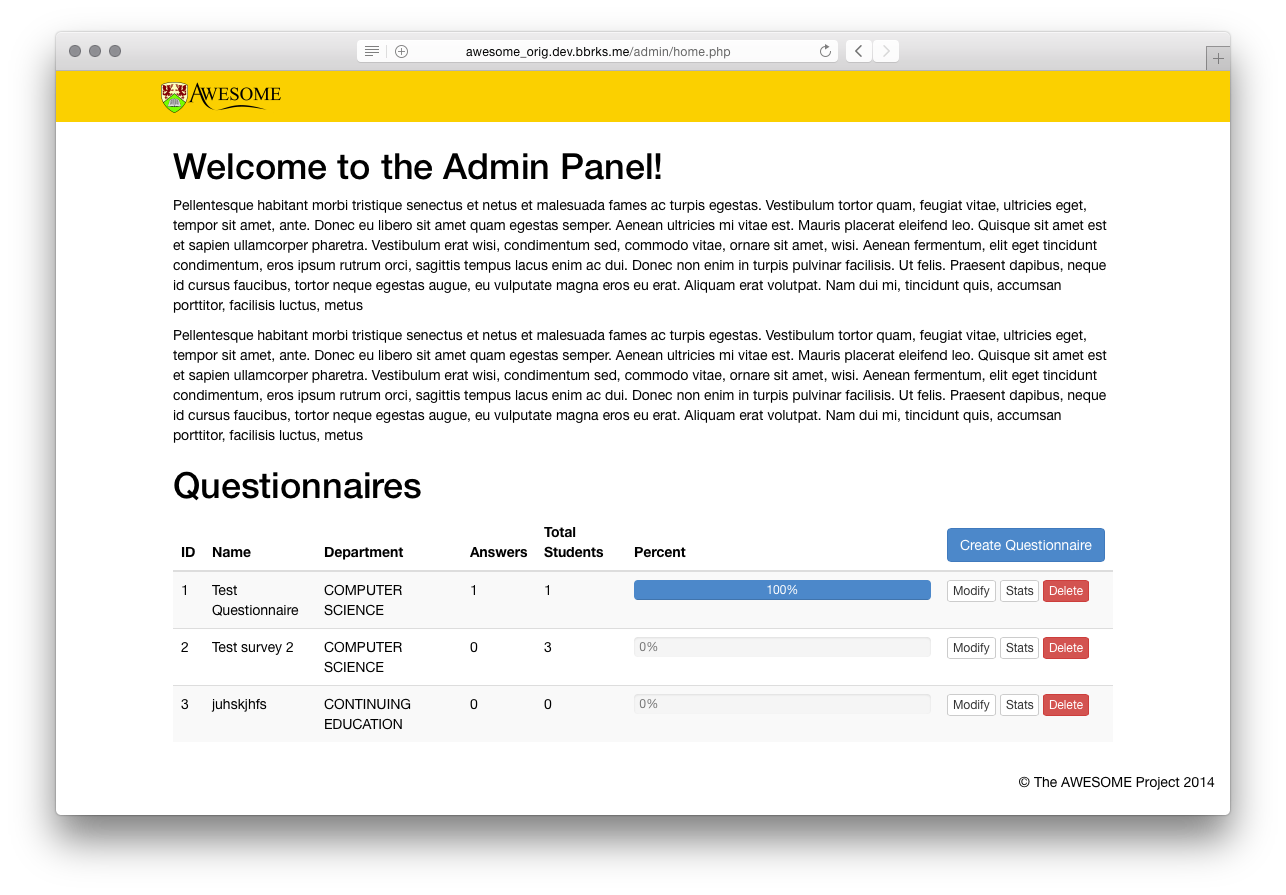
\includegraphics[width=\textwidth]{screens/prototype-viewall}
		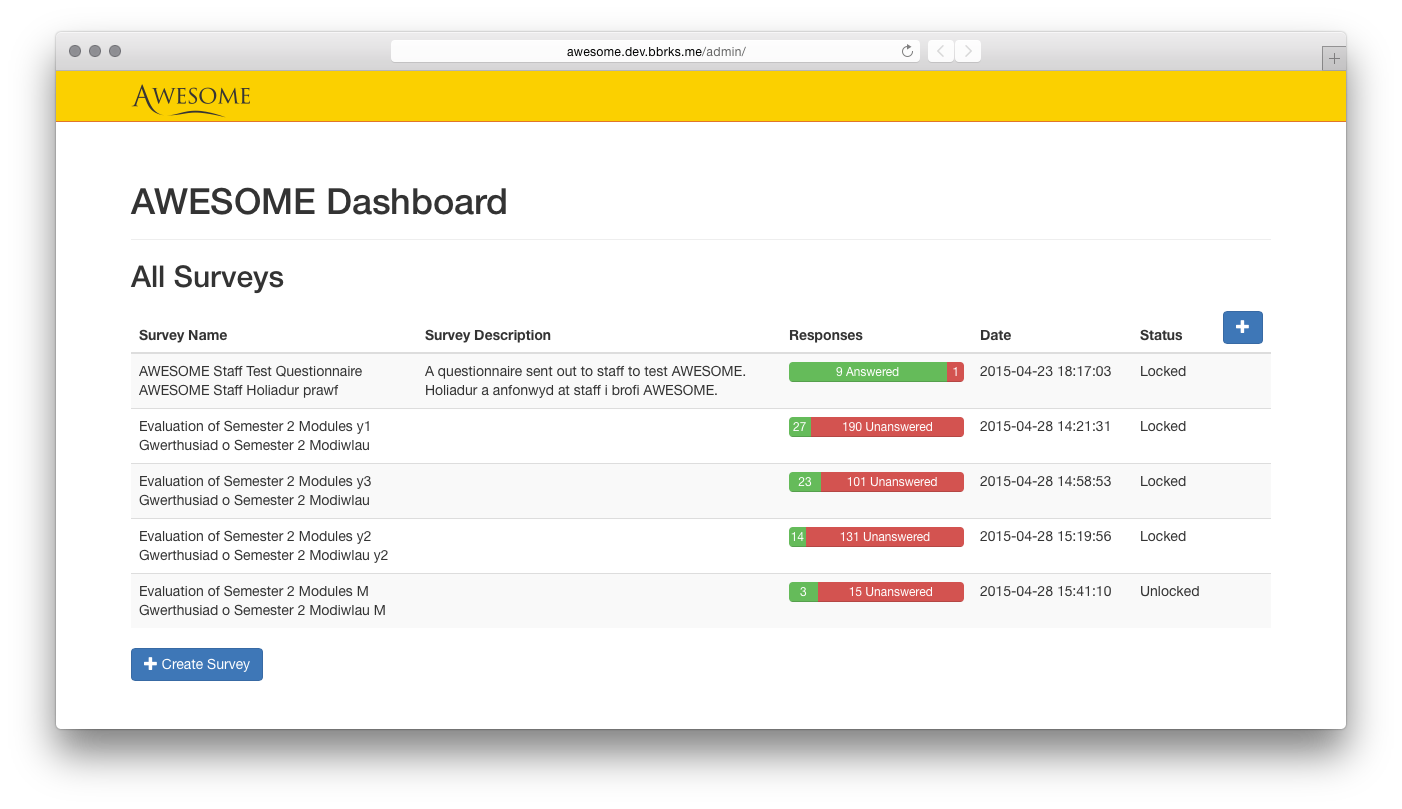
\includegraphics[width=\textwidth]{screens/final-viewall}
		\caption{A comparison of surveys view between the prototype version and the submitted version of \acs{AWESOME}}
		\label{fig:surveys-comparison}
	\end{figure}
	
	\begin{figure}[h]
		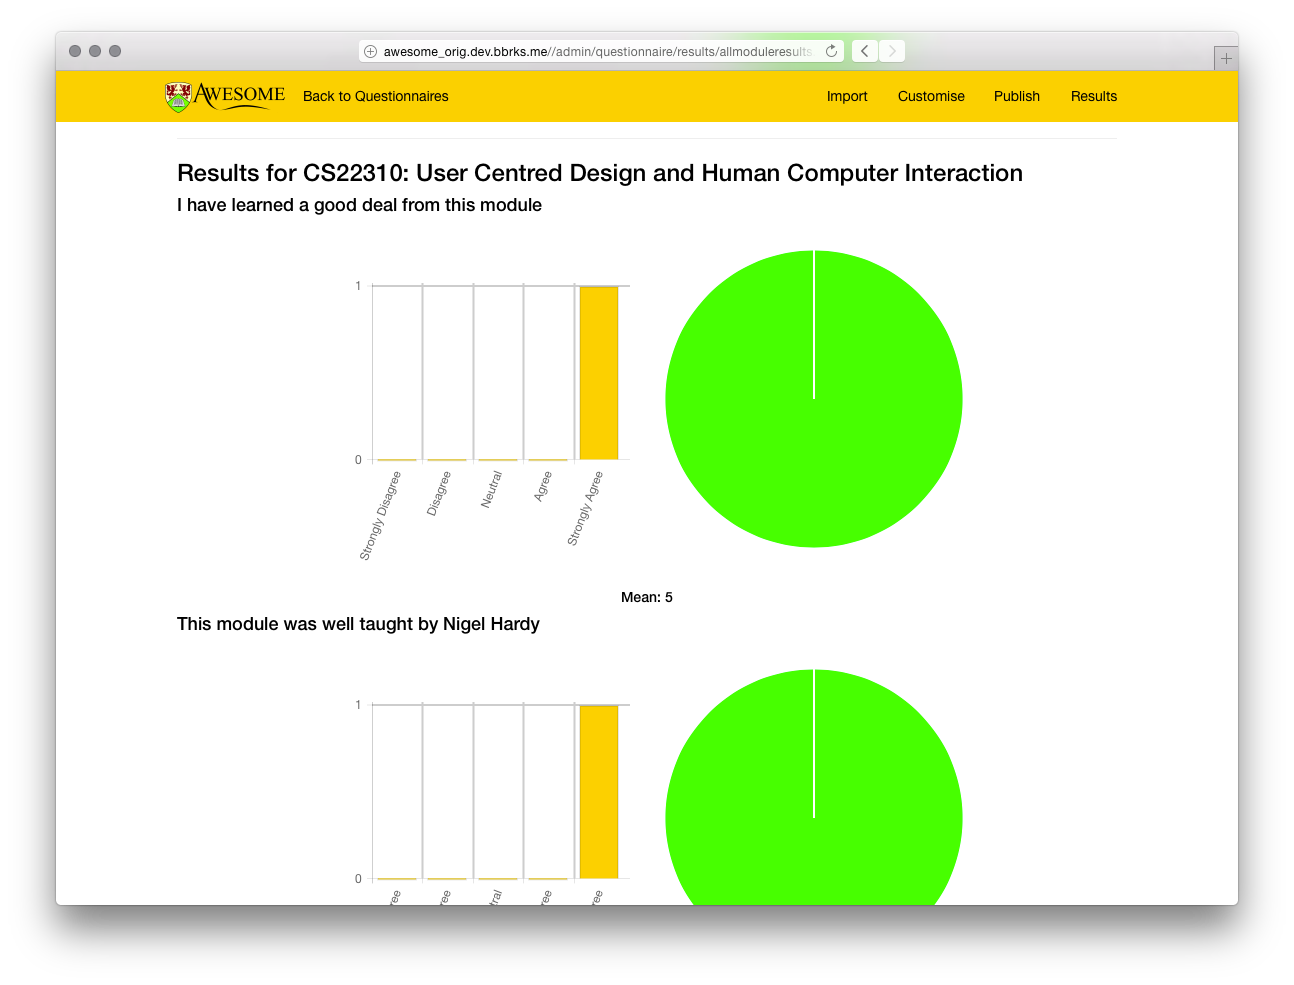
\includegraphics[width=\textwidth]{screens/prototype-results}
		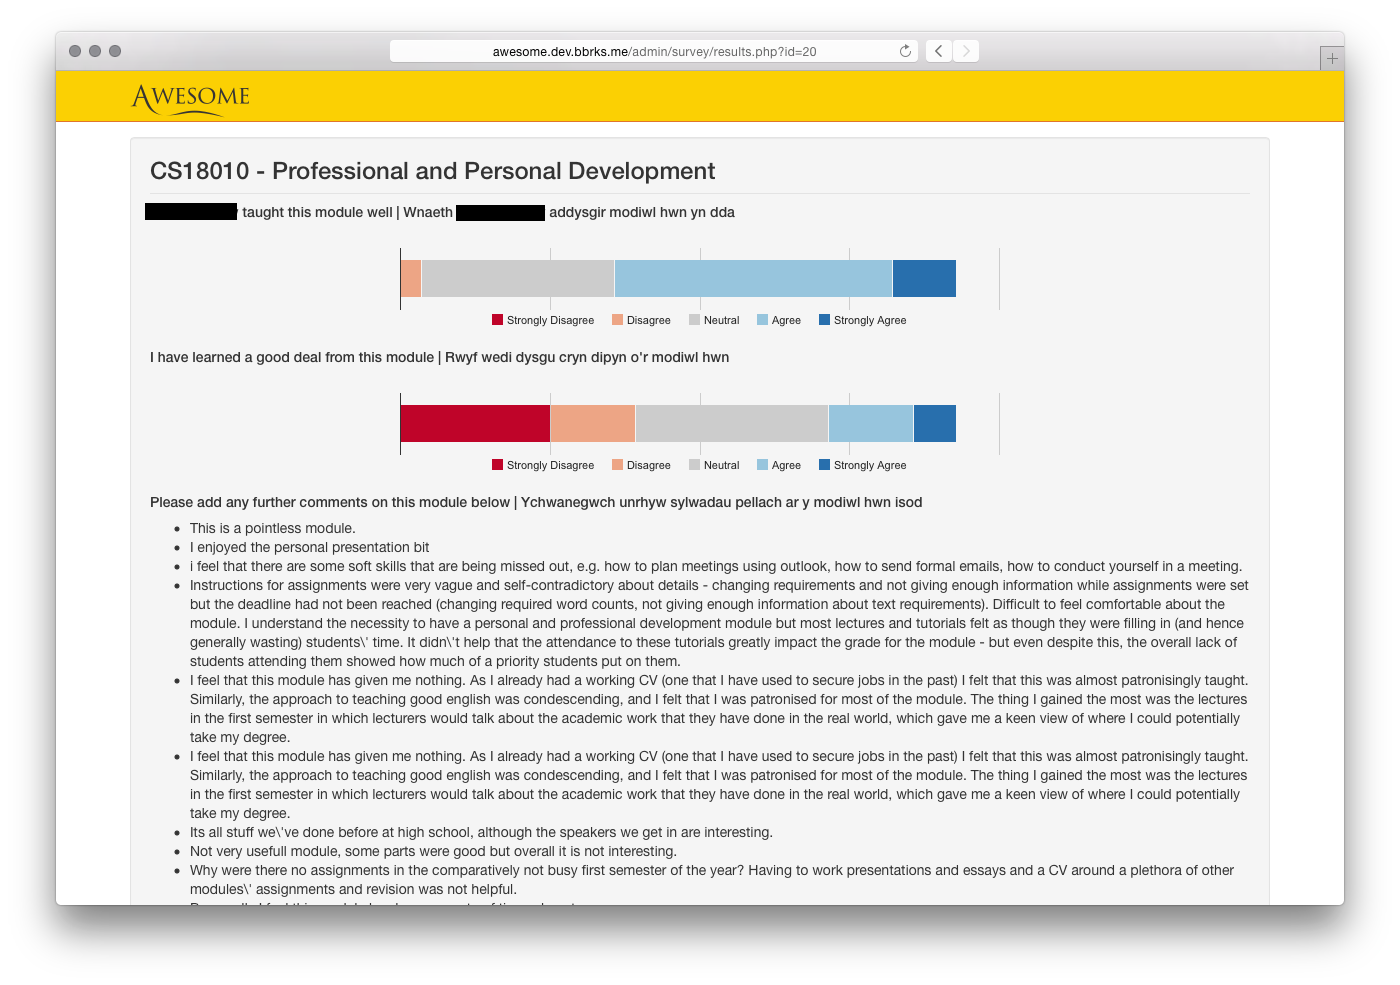
\includegraphics[width=\textwidth]{screens/final-results}
		\caption{A comparison of results between the prototype version and the submitted version of \acs{AWESOME}}
		\label{fig:results-comparison}
	\end{figure}
	
	\begin{figure}[h]
		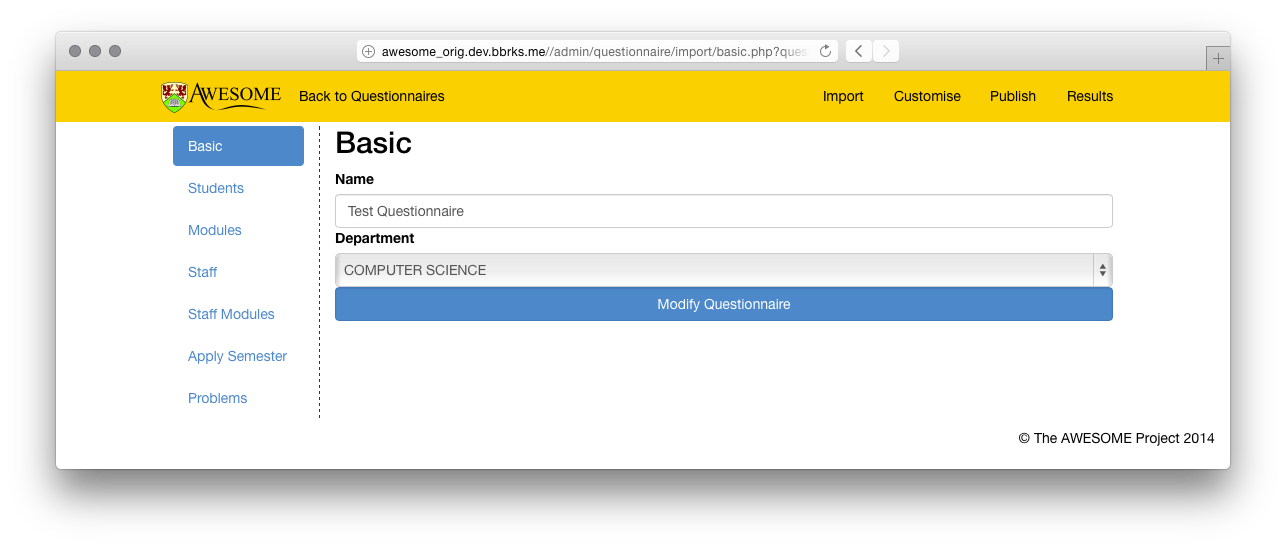
\includegraphics[width=\textwidth]{screens/prototype-single}
		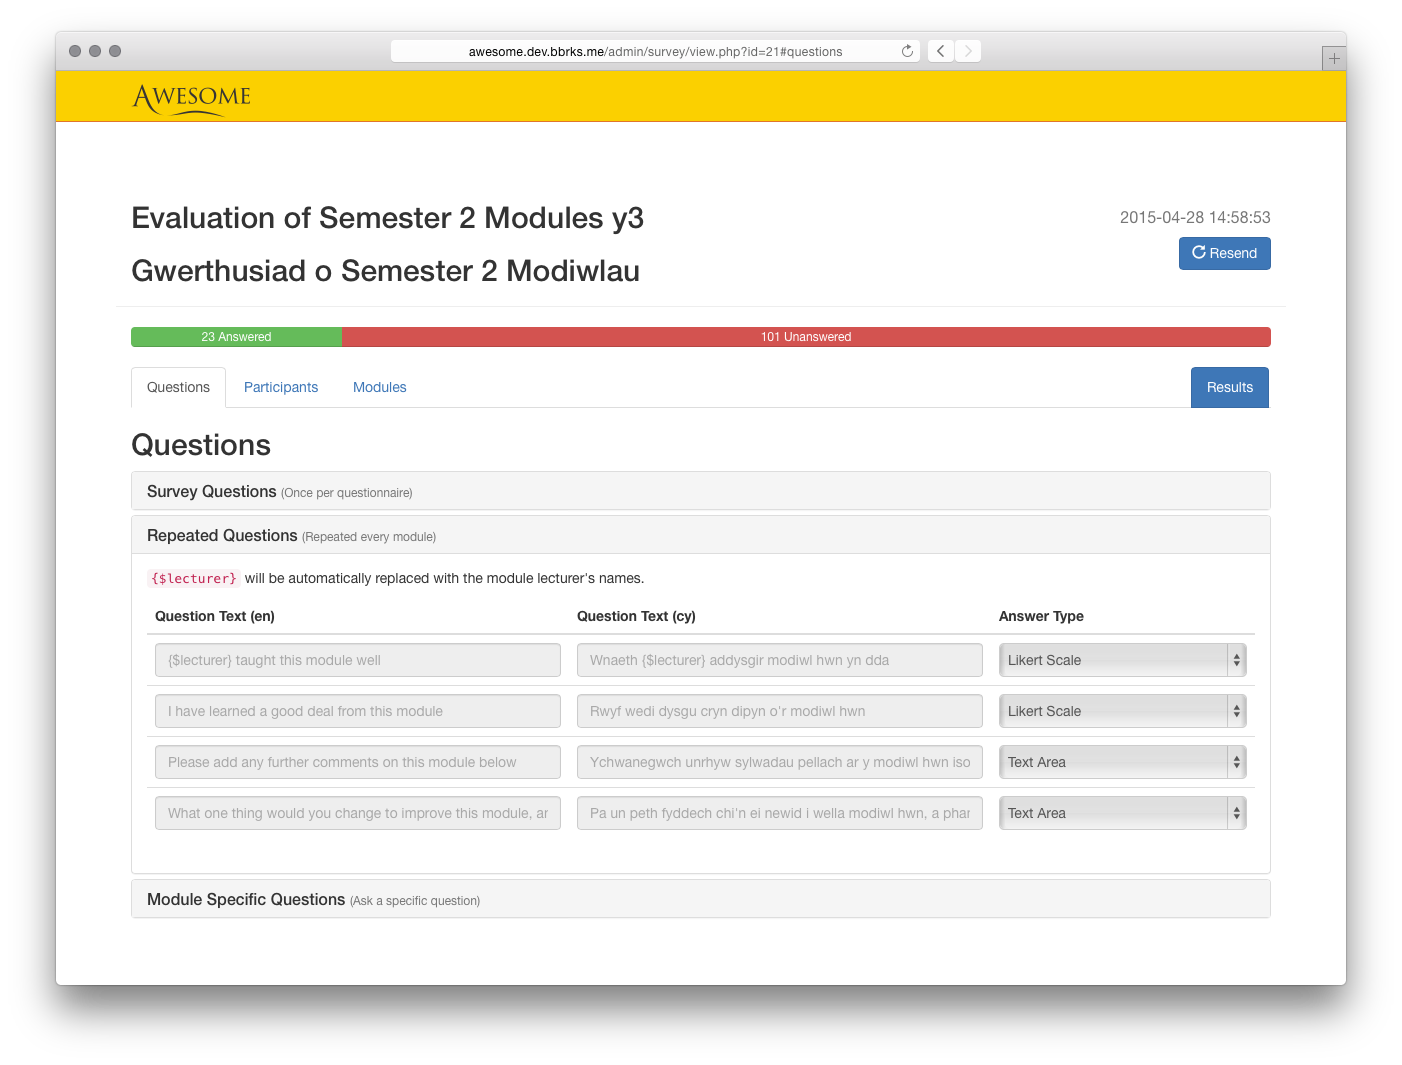
\includegraphics[width=\textwidth]{screens/final-questions}
		\caption{A comparison of survey view between the prototype version and the submitted version of \acs{AWESOME}}
		\label{fig:results-comparison}
	\end{figure}
	
	\begin{figure}[h]
		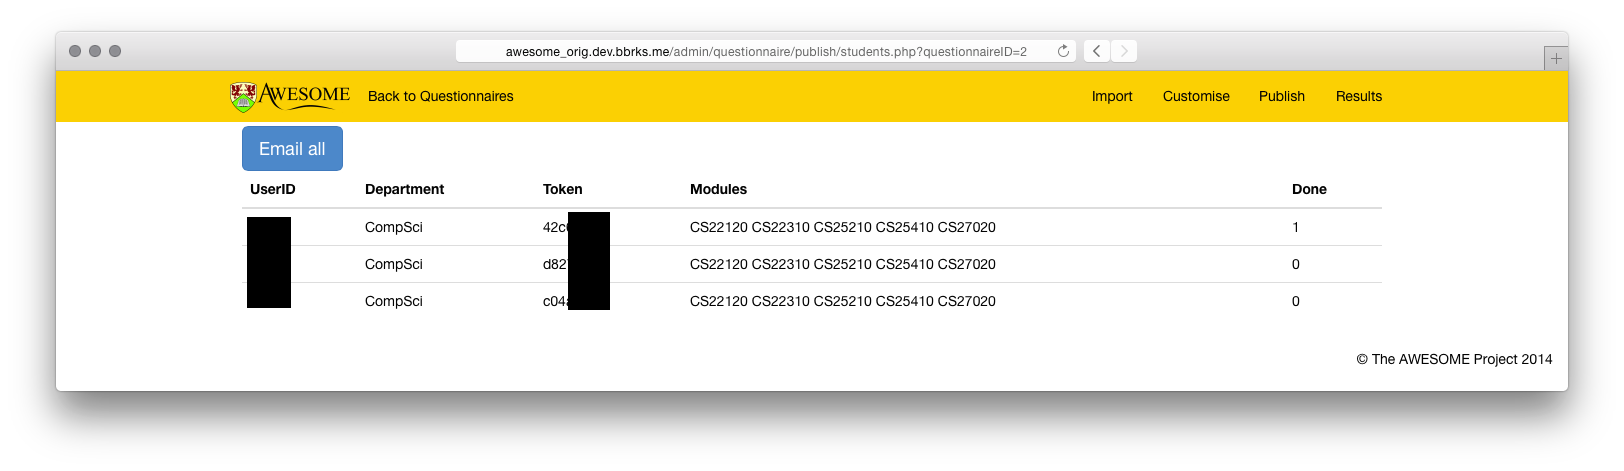
\includegraphics[width=\textwidth]{screens/prototype-respondents}
		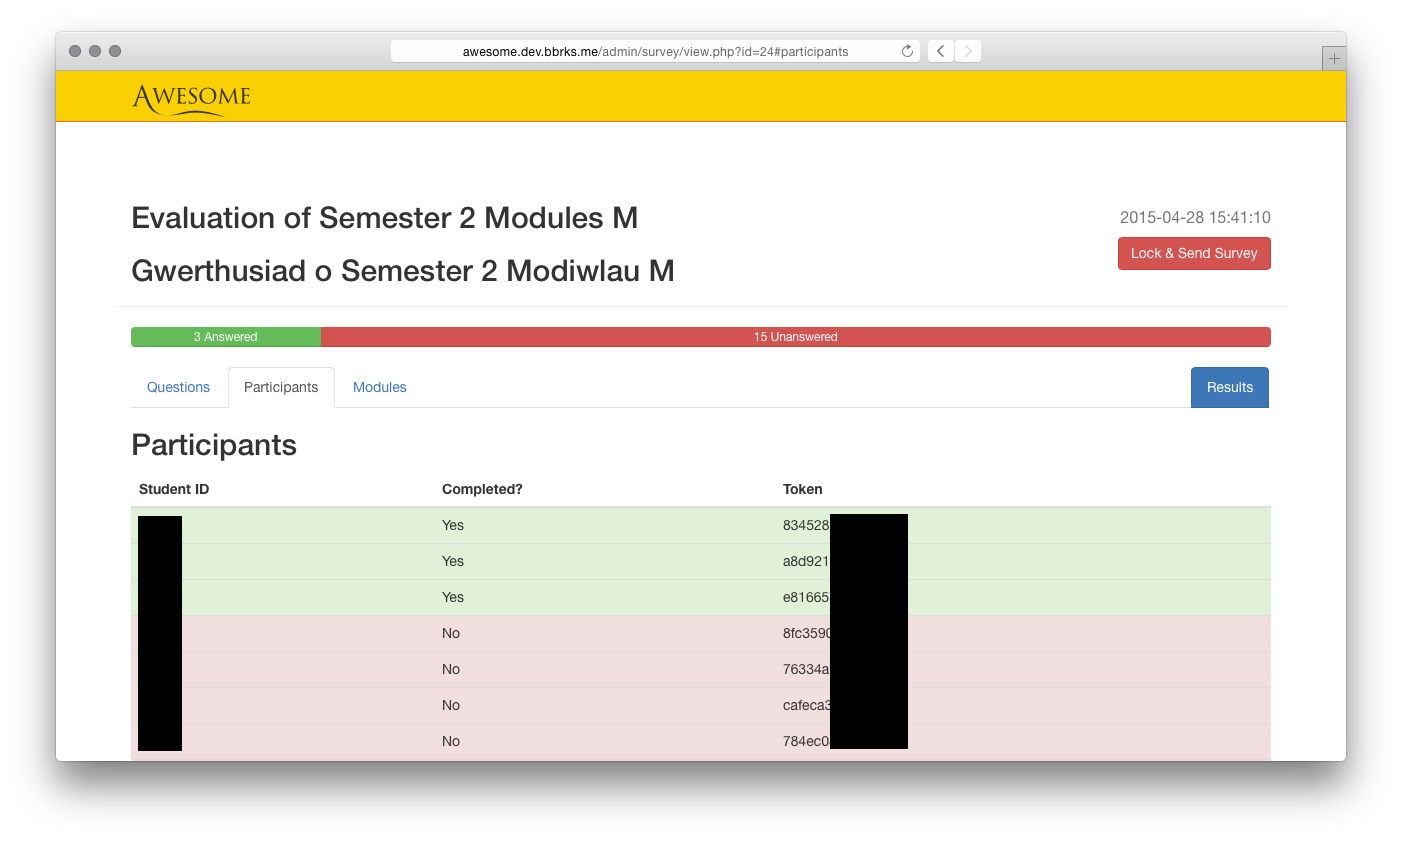
\includegraphics[width=\textwidth]{screens/final-respondents}
		\caption{A comparison of respondents between the prototype version and the submitted version of \acs{AWESOME}}
		\label{fig:results-comparison}
	\end{figure}